\documentclass{article}
% This is a LaTeX file.  It is a text file that is compiled
% by a program called LaTeX into a pretty PDF file.  
% If you're viewing this file on CoCalc, you'll see that PDF 
% in the window to the right.
%
% The LaTeX macro language is complicated, so we have inserted
% lots of documenting comments into the file.  Comments start
% with `%' and continue to the end of the line.  In CoCalc's
% window, they are colored brownish-red.
%
% Comments prefixed with `Student:' are relevant to students.
% Skip anything else you don't understand, or ask me.
%
% set font encoding for PDFLaTeX or XeLaTeX
\usepackage{ifxetex}
\ifxetex
  \usepackage{fontspec}
\else
  \usepackage[T1]{fontenc}
  \usepackage[utf8]{inputenc}
  \usepackage{lmodern}
\fi

% Student: These lines describe some document metadata.
\title{Problem Set 2}
\author{%
% Student: change the next line to your name!
    Name
\\  MATH-UA 120 Discrete Mathematics
}
\date{due October 7, 2022 at 11:00pm}


\usepackage[headings=runin-fixed-nr]{exsheets}
% These make enumerates within questions start at the second ("(a)") level, rather than the first ("1.") level.
\makeatletter
    \newcommand{\stepenumdepth}{\advance\@enumdepth\@ne}
\makeatother
\SetupExSheets{
    question/pre-body-hook=\stepenumdepth,
    solution/pre-body-hook=\stepenumdepth,
}
\DeclareInstance{exsheets-heading}{runin-nn-np}{default}{
    runin = true,
    title-post-code = .\space,
    join = {
        main[r,vc]title[l,vc](0pt,0pt);
    }
}
\newif\ifshowsolutions
% Student: replace `false' with `true' to typeset your solutions.
% Otherwise they are ignored!
\showsolutionstrue
\ifshowsolutions
    \SetupExSheets{
        question/pre-hook=\itshape,
        solution/headings=runin-nn-np,
        solution/print=true,
        solution/name=Answer
    }%
    \makeatletter%
    \pretocmd{\@title}{Answers to }%
    \makeatother%
\else
    \SetupExSheets{solution/print=false}
\fi

% Bug workaround: http://tex.stackexchange.com/a/146536/1402
%\newenvironment{exercise}{}{}
\RenewQuSolPair{question}{solution}
%\let\answer\solution
%\let\endanswer\endsolution
\usepackage{manfnt}
\newcommand{\danger}{\marginpar[\hfill\dbend]{\dbend\hfill}}

\usepackage{subcaption}

\newcommand{\Z}{\mathbb{Z}}
\newcommand{\R}{\mathbb{R}}
\newcommand{\N}{\mathbb{N}}
\newcommand{\Q}{\mathbb{Q}}

\usepackage{amsmath, amsthm}
\usepackage{amsfonts}
\usepackage{siunitx}
\DeclareSIUnit\pound{lb}
\usepackage{hyperref}
\newtheorem*{theorem}{Theorem}
\newtheorem*{proposition}{Proposition}
\theoremstyle{definition}
\newtheorem*{definition}{Definition}
% We are creating a command "\xor".
\newcommand{\xor}{\underline{\lor}}
% This is the beginning of the part of the file that describes
% the text of the document.
% That's why it says `\begin{document}' below. :-)
\begin{document}
\maketitle



These are to be written up \LaTeX and turned in to Gradescope.\\



\ifshowsolutions
    \SetupExSheets{solution/print=true}
\else
    \danger
 \underline{ \LaTeX  Instructions:}  You can view the source (\texttt{.tex}) file to get some more examples of \LaTeX{} code.  I have commented the source file in places where new \LaTeX{} constructions are used.
  
  Remember to change \verb|\showsolutionsfalse| to \verb|\showsolutionstrue|
    in the document's preamble 
    (between \verb|\documentclass{article}| and \verb|\begin{document}|)
\fi

\section*{Assigned Problems}

\begin{question}
Consider a group consisting of 3 dogs and 3 cats. Answer the following questions, giving a quick explanation in each case.

\begin{enumerate}
	\item In how many ways can they all sit in a row? In how many ways can they sit in a row if the dogs sit together and the cats sit together?
	\item In how many ways can they sit in a row if only the dogs are required to sit together?
	\item In how many ways can they sit in a row if no two animals of the same species are allowed to sit next to each other?
	\item In how many ways can the animals sit together around a round table? Here, the only thing that matters is who is sitting next to whom.
\end{enumerate}
\end{question}
% Student: put your answer between the next two lines.
\begin{solution}
\begin{enumerate}
	\item For the first part, there are $6$ choices for the first animal, $5$ for the second one, and so on, for the total of $6!$. For the second part, there are $3!$ ways to order the dogs, $3!$ ways to order the cats, and they can sit with dogs first then cats, or vice-versa, for a total of $2 \times (3!)^2$ ways.
	
	\item There are $3!$ ways to order the dogs, $3!$ ways to order the cats, and for each such orders, we can have the configurations $DDDCCC$, $DCCCDD$, $DDCCCD$, and $CCCDDD$, for a total of $4 \times (3!)^2$ ways.
	
	\item We have 6 choices for the first animal, then 3 choices for the second one (since they have to be of a different species), then 2 choices for the third one, 2 for the fourth one, and one choices for the two remaining ones, for a total of $6 \times 3 \times 2^2$.
	
	\item There are $6!$ to choose an ordering around the table. However, each order $ABCDEF$ is the same as $BCDEFA$, $CDEFAB$, \dots, when sitting around a round table. This leaves a total of $6! / 6 = 5!$ possible ways.
	
    \textbf{Alternate acceptable solution:} If we do not care about keeping track of who is sitting on the right and on the left of each animal, then reversing the order makes no difference: we regard $ABCDEF$ as the ``same seating arrangement'' as $FEDCBA$, since in both cases, for each animal, the same two other animals are sitting in adjacent seats. In this case we would divide the previous answer by 2 to obtain $5! / 2 = 60$ possible ways.
	
\end{enumerate}
{\color{red} Rubric:
\begin{itemize}
\item 2.5P for each part
\item Grader: Please expand on rubric yourself.
\end{itemize}}
\end{solution}


\begin{question}
    The internet is a network of interconnected computers. Each computer interface on the Internet is identified by an Internet address. In IPv4 (Internet Protocol, Version 4), the addresses are divided into five classes -- Classes A through Classes E. Only Classes A, B, and C are used to identify computers on the Internet.
    
    A Class A address is a bit string of length 32. A bit string consists of $0$'s and $1$'s. The first bit is 0 (to identify it as a Class A address). The next 7 bits, called the \textit{netid}, identify the network. The remaining 24 bits, called the \textit{hostid}, identify the computer interface. The netid must not consist of all 1's. The hostid must not consist of all 0's or all 1's. How many Class A Internet addresses are there?
\end{question}
% Student: put your answer between the next two lines.
\begin{solution}
Let's consider the total of all possible lists first. There are $2^7$ total 7-bit strings for the netid and $2^{24}$ 24-bit strings for the hostid. Since all $1$'s are not allowed as a netid, there are $2^7-1$ netids. Since the strings of all $1$'s and all $0$'s are not allowed, there are $2^{24}-2$ hostids. By the Multiplication Principle, there are 
\[
(2^7-1)(2^{24}-2)
\]
Class A Internet addresses.
{\color{red} Rubric:
\begin{itemize}
\item 2P for each part of answer
\item 2P for explanation
\item Grader: Please expand on rubric yourself.
\end{itemize}}
\end{solution}


\begin{question}
   (Scheinerman, Exercise 10.11:)
   Let $a$ and $b$ be integers, and let $A = \{x \in \Z ~:~ a|x\}$ and $B = \{ x\in\Z ~:~ b|x\}$.  
   Find and prove a necessary and sufficient condition for $A \subseteq B$.
   (That is, find some condition in terms of $a$ and $b$ such that the statement\\~\\
   $~~~$ ``$A \subseteq B$ if and only if [the condition involving $a$ and $b$ you provide is satisfied]''\\~\\
   is true.  Then, prove this if-and-only-if statement.)
\end{question}
% Student: put your answer between the next two lines.
\begin{solution}
We make the following claim:
\begin{proposition}
Let $a$ and $b$ be integers, and let $A = \{x \in \Z ~:~ a|x\}$ and $B = \{ x\in\Z ~:~ b|x\}$.  
$A \subseteq B$ if and only if $b|a$.
\end{proposition}
\begin{proof}
($\Rightarrow$) First, we show that if $A\subseteq B$, then $b|a$.

Consider an arbitrary element $x \in A$.  This means that $x$ is an integer and $a|x$.  So, there is an integer $m$ such that $x = am$.  Note that since $x$ is an arbitrary element of $A$, $m$ could be any integer.

We know that any such $x$ is also an element of $B$ since $A \subseteq B$.  So, $b$ divides $am$, for \emph{any} integer $m$ (including when $m$ is prime).

In particular, if $m = 1$, there must be some $n$ such that $a = bn$.  This means that $b$ must in fact divide $a$.

($\Leftarrow$) Next, we show that if $b|a$, then $A\subseteq B$.

Suppose that $b |a$.  This means that $a = bm$ for some integer $m$.

Next, consider an arbitrary element $x \in A$.  So, $x$ is an integer and $a|x$.  So, there is some integer $k$ such that $x = ak = (bm)k = b(mk)$.

Since $mk$ is an integer and $x = b(mk)$, then $b|x$.  Therefore, $x \in B$.

This shows that $A \subseteq B$.
\end{proof}
{\color{red} Rubric:
\begin{itemize}
\item Follow RVF rubric with 1P for correct claim
\end{itemize}}
\end{solution}

\begin{question}
Describe explicitly in English the following sets, then give their cardinality.

\begin{enumerate}
	\item $\{x \in 2^{\Z} : 5 \in x \}$
	\item $\{x \in 2^{\Z} : x \subseteq \{ 1, 2, 3\} \}$
	\item $\{x \in 2^{\Z} : x \subseteq \{ 1, 2, \{3, 4\} \} \}$
	\item $\{x \in 2^{\Z} : x \in \{ 1, 2, \{3, 4\} \} \}$
	\item $\{x \in 2^{\Z} : y \in x \implies y = 0 \}$
\end{enumerate}
\end{question}
% Student: put your answer between the next two lines.
\begin{solution}
\begin{enumerate}
	\item This is the set of all subsets of $\Z$ that contain $5$. There are infinitely many such subsets, like $\{5\}, \{5,6\}, \{5,6, 7\}, \dots$, so $\left | \{x \in 2^{\Z} : 5 \in x \} \right |$ is infinite.
	\item This is the set of all subsets of $\Z$ that are also subsets of $\{1, 2, 3\}$, so it is actually the set of all subsets of $\{1,2,3\}$. Therefore
	\[
	\left |\{x \in 2^{\Z} : x \subseteq \{ 1, 2, 3\} \} \right | = \left | 2^{\{1, 2, 3\}} \right | = 2^{|\{ 1, 2, 3\}|} = 2^3 = 8.
	\]
	
	\item This is the set of all subsets of $\Z$ that are also subsets of $ \{ 1, 2, \{3, 4\} \} \}$. But $\{ 3, 4 \}$ is not an element of $\Z$, so it means that set in question is the set of all subsets of $\{1,2\}$. Therefore, as above, 
	\[
	\left |\{x \in 2^{\Z} : x \subseteq \{ 1, 2, \{3, 4\} \} \} \right | = 2^{|\{1,2 \}|} = 2^2 = 4.
	\]
	
	\item This is the set of all subsets of $\Z$ that are also elements of $ \{ 1, 2, \{3, 4\} \} \}$. But out of these elements, there is only one subset of $\Z$, namely $\{ 3, 4 \}$, and therefore the set in question is the set $\{ \{3,4\} \}$, which contains the one element $\{3,4\}$. Therefore
	\[
	\left | \{x \in 2^{\Z} : x \in \{ 1, 2, \{3, 4\} \} \} \right | = 1.
	\]
	
	\item This is the set of all subsets of $\Z$ such that if there is an element in the subset, then it is $0$. In other words, such a subset can only contain the element $0$, so it is $\{ 0 \}$... or $\emptyset$! Therefore, the set in question is $\{ \emptyset, \{0\}\}$, and thus
	\[
	\left | \{x \in 2^{\Z} : y \in x \implies y = 0 \} \right | = 2.
	\]
\end{enumerate}
{\color{red} Rubric:
\begin{itemize}
\item 2P for each part
\item Grader: Please expand on rubric yourself.
\end{itemize}}
\end{solution}


\begin{question}
\begin{enumerate}
	\item For each of the following statements, describe it in English, and say if it is true or false (without proof). Then write its negation using quantifier, and express this negation in English. For instance, the statement $\forall x \in \Z \; x < 0$ means every integer is negative, and it is false. Its negation is $\exists x \in \Z \; x \geq 0$, which means that there exists a nonnegative integer.
	
	\begin{enumerate}
		\item $\forall x \in \Z \; \forall y \in \Z \; x + y = 0$
		\item $\forall x \in \Z \; \exists y \in \Z \; x + y = 0$
		\item $\forall n \in \Z \; \exists k \in \Z \; \exists d \in \Z \; k+ n = 2d$
		\item $\exists n \in \Z \; \forall k \in \Z \; \exists d \in \Z \; k+ n = 2d$
	\end{enumerate}
	
	\item For each of the statements (c) and (d): prove it if it is true, or prove the negation if it is false. These proofs are short.
\end{enumerate}
\end{question}
% Student: put your answer between the next two lines.
\begin{solution}
\begin{enumerate}
	\item 
	\begin{enumerate}
		\item The statement means that the sum of any two integers is 0. This is false. Its negation is
		\[
		\exists x \in \Z \; \exists y \in \Z \; x + y \neq 0
		\]
		which means that we can find two integers whose sum is not zero.
		
		\item The statement means to any integer, we can add another integer to get 0. This is true. Its negation is
		\[
		\exists x \in \Z \; \forall y \in \Z \; x + y \neq 0
		\]
		which means that we can find an integer such that, regardless of what other integer we add to it, we never get a sum equal to 0.
		
		
		\item The statement means that to any integer, we can add another integer to get an even number. This is true. Its negation is
		\[
		\exists n \in \Z \; \forall k \in \Z \; \forall d \in \Z \; k + n \neq 2d.
		\]
		which means that we can find an integer such that, regardless of what other integer we add to it, we will never get an  even sum.
		
		\item The statement means that there exists an integer such that, regardless of what other integer we add to it, we always get an even sum. This is false. Its negation is
		\[
		\forall n \in \Z \; \exists k \in \Z \; \forall d \in \Z \; k + n \neq 2d.
		\]
		which means that to any integer, we can add another integer and get a sum which is not even.
		
	\end{enumerate}
	\item \begin{itemize}
		\item For part (c): Let us show that
		\[
		\forall n \in \Z \; \exists k \in \Z \; \exists d \in \Z \; k + n = 2d
		\]
		Let $n \in \Z$. Take $k = n$ and $d = n$. Then $k+n = n + n = 2n = 2d$.
		
		\item For part (d): Let us show that
		\[
		\forall n \in \Z \; \exists k \in \Z \; \forall d \in \Z \; k + n \neq 2d
		\]
		Let $n \in \N$. Take $k = n + 1$. Then $k + n = n+1+n = 2n + 1$ is odd, so it is not even, that is, it cannot be written as $2d$ for any $d \in \Z$.
		
	\end{itemize}
	
\end{enumerate}

{\color{red} Rubric:
\begin{itemize}
\item Part a: 1.5P for each part
\item Part b: 2P for each part
\item Grader: Please expand on rubric yourself.
\end{itemize}}
\end{solution}



\begin{question}
    (Scheinerman, Exercise 12.3:)
    Let $A$ and $B$ be sets with $|A| = 10$ and $|B| = 7$.
    What can we say about $|A\cup B|$?
    
    In particular, find two numbers $x$ and $y$ for which we can be sure that $x \leq |A \cup B| \leq y$ and then find specific sets $A$ and $B$ so that $|A \cup B| = x$ and another pair of sets so that $|A \cup B| = y$.
    
    Finally, answer the same question about $|A\cap B|$.  
\end{question}
% Student: put your answer between the next two lines.
\begin{solution}
    By Proposition 12.4 in the text:
    \[
        |A\cup B| = |A| + |B| - | A \cap B| = 17 - |A \cap B|
    \]
    Now $A \cap B$ is a subset of $B$, so it can have most $7$ elements.
    It could also be empty, in which case it can have zero elements.
    So
    \[
        0 \leq |A \cap B| \leq 7
    \]
    This means that 
    \[
       17-0 \geq 17 - |A \cap B| \geq 17-7
    \]
    and therefore 
    \[
        10 \leq |A \cup B| \leq 17
    \]
    To be specific, let $A = \{1,2,\dots,10\}$.
    If $B = \{1,2,\dots,7\}$, then $|A \cup B| = |A| =10$ and $|A \cap B| = |B| = 7$.
    If instead $B = \{11,12,\dots,17\}$, then $|A \cup B| = 17$ and $|A \cap B| = 0$.

{\color{red} Rubric:
\begin{itemize}
\item Follow RVF rubric with 1P for answer
\end{itemize}}
\end{solution}


\begin{question}
   Let $I=\{1, 2, \dots, n\}$. Given a collection of sets $\{A_1,A_2,\dots, A_n\}$, denoted by $\{A_i\}_{i\in I}$. $\{A_i\}_{i\in I}$ is said to be \textbf{disjoint} if $\cap_{i\in I}A_i=\emptyset$, and it is said to be \textbf{pairwise disjoint} if $A_i\cap A_j=\emptyset$ whenever $i\neq j$. What is the difference between a \textbf{disjoint} collection of sets and a \textbf{pairwise disjoint} collection of sets? (\textit{Draw a picture to convince yourself.}) Give an example of a collection of sets that is disjoint, but not pairwise disjoint. (\textit{Hint: You need a minimum of three sets.})
\end{question}
% Student: put your answer between the next two lines.
\begin{solution}
A collection of sets is \textbf{disjoint} if there is no element shared by all sets in the collection; whereas, a collection of sets is \textbf{pairwise disjoint} if no two sets (that are different) share a common element. For example, in the following diagrams, the first picture is disjoint, but not pairwise disjoint and the second picture is pairwise disjoint.
\begin{figure}[h]
\centering
	\begin{subfigure}[h]{.35\textwidth}
	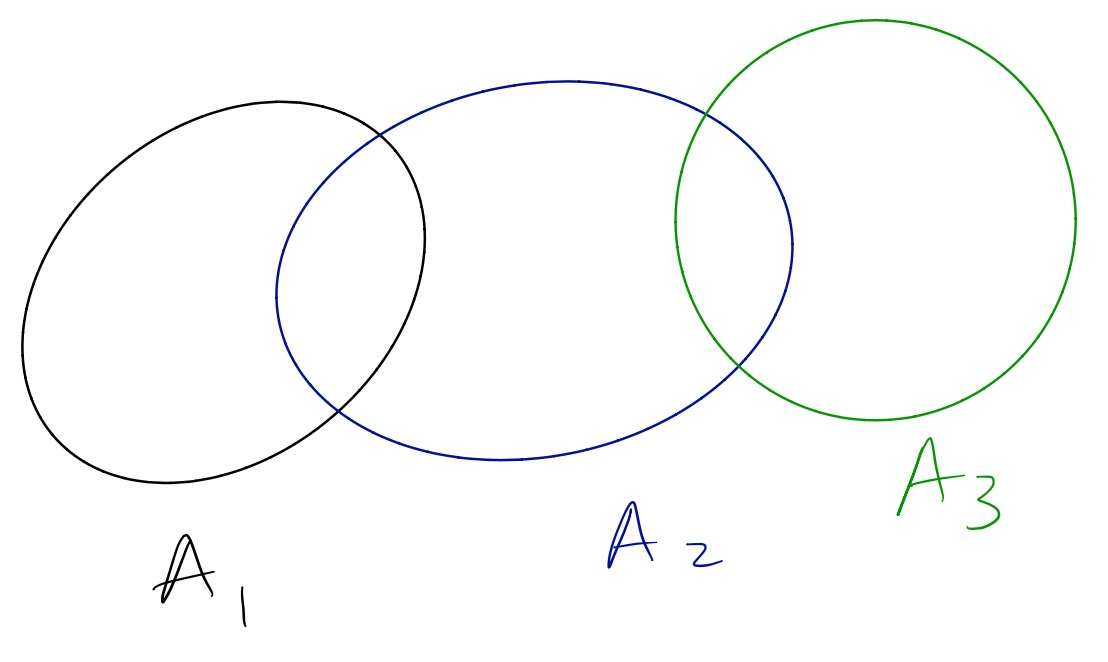
\includegraphics[width=\textwidth]{ProblemSets/fig/disjoint.jpg}
	\caption{Disjoint but not pairwise disjoint}
	\end{subfigure}
	~\quad\hspace{1cm}
	\begin{subfigure}[h]{.35\textwidth}
	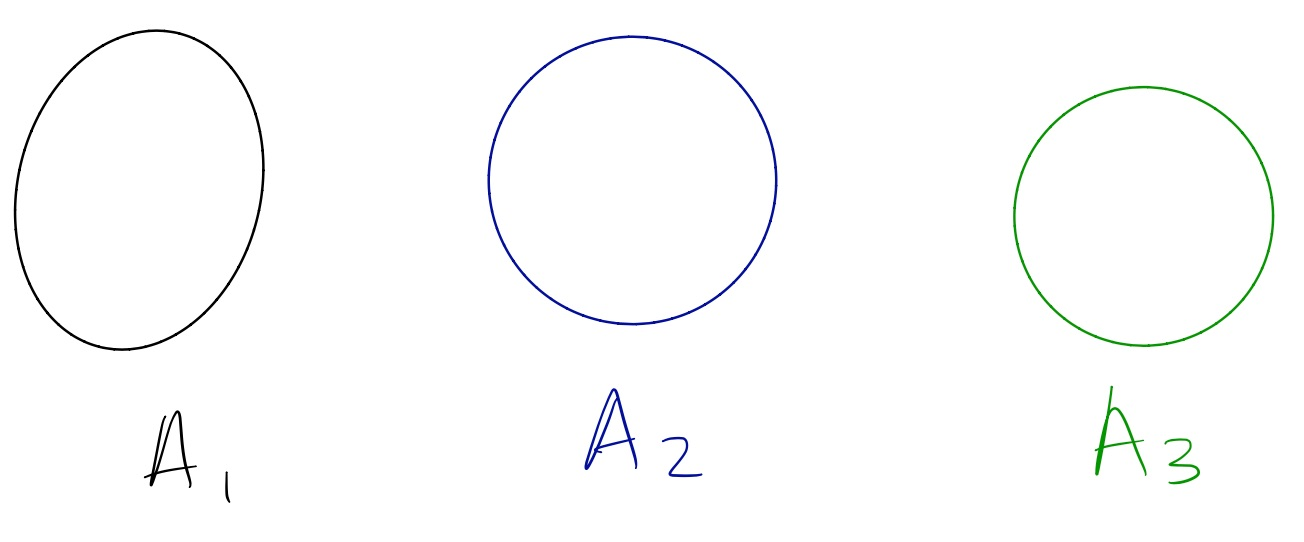
\includegraphics[width=\textwidth]{ProblemSets/fig/pair-disjoint.jpg}
	\caption{Pairwise disjoint}
	\end{subfigure}	
\end{figure}


\textbf{Example:} Let $A_1=\{1, 2, 3, 4\}, A_2=\{3, 4, 5, 6\}$ and $A_3=\{1, 6, 7\}$.
\begin{itemize}
\item Notice that 
\begin{align*}
A_1\cap A_2\cap A_3 &= (A_1\cap A_2)\cap A_3\\
&=\{3,4\}\cap A_3\\
&=\emptyset.
\end{align*} Hence they are disjoint.
\item However,
\begin{align*}
A_1\cap A_2 &=\{3, 4\}\\
A_1\cap A_3 &=\{1\}\\
A_2\cap A_3 &=\{6\},
\end{align*}
which is not pairwise disjoint.
\end{itemize}

{\color{red} Rubric:
\begin{itemize}
\item 5P for explanation
\item 5P for example and explanation of example.
\end{itemize}}
\end{solution}


\begin{question}
   (Scheinerman, Exercise 12.19:)
   Prove:
   \[ A-(B\cup C)=(A-B)\cap(A-C).\]
\end{question}
% Student: put your answer between the next two lines.
\begin{solution}
\begin{proof}
We will prove $A-(B\cup C) = (A-B)\cap(A-C)$, by first proving $A-(B\cup C) \subseteq (A-B)\cap(A-C)$ and then $(A-B)\cap(A-C)\subseteq A-(B\cup C)$.
\begin{enumerate}
\item[($\subseteq$)] Suppose $x\in A-(B\cup C)$. By definition, $x\in A$, but $x\notin B\cup C$. If $x\notin B\cup C$, then $x\notin B$ and $x\notin C$. Since $x\in A$ but $x\notin B$, $x\in A-B$. Similarly, since $x\in A$ but $x\notin C$, $x\in A-C$. Since $x\in A-B$ and $x\in A-C$, we conclude $x\in (A-B)\cap(A-C)$.

\item [($\supseteq$)] Suppose $x\in (A-B)\cap(A-C)$. By definition, $x\in A-B$ and $x\in A-C$. Since $x\in A-B$, $x\in A$ but $x\notin B$. Since $x\in A-C$, $x\in A$ but $x\notin C$. Since $x\notin B$ and $x\notin C$, then $x\notin B\cup C$. Since $x\in A$ and $x\notin B\cup C$, we conclude that $x\in A-(B\cup C)$.
\end{enumerate}
Therefore, $A-(B\cup C) = (A-B)\cap(A-C)$.
\end{proof}
{\color{red} Rubric:
\begin{itemize}
\item Follow RVF rubric with 1P for \LaTeX
\end{itemize}}
\end{solution}


\begin{question}
    Let $n$ be a positive integer.  Give a combinatorial proof of the identity:
    \[ n^3 = n(n-1)(n-2) + 3n(n-1) + n. \]
\end{question}
% Student: put your answer between the next two lines.
\begin{solution}
    Let $S$ denote the set of all $3-$lists where each element is from the set $\{1, 2, \dots, n\}$:
    \[S=\{(a_1, a_2, a_3): a_1, a_2, a_3\in \{1, 2, \dots, n\}\}.\]
    We would like to count the number of elements of the set $S$ (ie, $|S|$).
    
    Answer 1: Since there are $n$ choices for each of the 3 positions in the list and repetition is allowed, there are $n^3$ total possible such lists.
    
    Answer2: Let $S_i$ be the set of $3-$lists where $i$ elements from each list are the same and $i\in\{1, 2, 3\}$. $S_1$ consists of $3-$lists where all elements are distinct (ie. no repetition), then there are $(n)_3=n(n-1)(n-2)$ total possible such lists. $S_2$ consists of $3-$lists where exactly 2 elements are the same. Note that there are 3 possible positions for the third different element in the 3-list. Since there are $n$ choices for the 2 elements that are the same, there are $n-1$ choices for the third different element. Then $|S_2|=3n(n-1)$. $S_3$ consists of $3$-lists where all three elements are the same; so there are $n$ total possible such lists. Since $S_1\cup S_2\cup S_3=S$ and $S_1, S_2,$ and $S_3$ are pairwise disjoint, $|S| = |S_1|+|S_2|+|S_3|= n(n-1)(n-2)+3n(n-1)+n$.
    
    Therefore, both $n^3$ and $n(n-1)(n-2)+3n(n-1)+n$ are the number of elements in $S$. So it must be the case that
    \[n^3 = n(n-1)(n-2) + 3n(n-1) + n. \]
    
{\color{red} Rubric:
\begin{itemize}
\item Follow RVF rubric with 1P for \LaTeX
\end{itemize}}
\end{solution}

\begin{question}
    Prove, combinatorially, that
    \[ 2 \cdot 3^0 + 2 \cdot 3^1 + 2 \cdot 3^2 + \ldots + 2 \cdot 3^{n-1} = 3^n - 1. \]
\end{question}
% Student: put your answer between the next two lines.
\begin{solution}
Suppose that $S$ denote the set of all $n$-integer lists where each element is from the numbers $0, 1, 2$, except for the list $(0, 0, \ldots, 0)$:
\[ S = \{ (a_1, a_2, \ldots a_n) ~:~ a_1, \ldots, a_n \in \{0, 1, 2\} \} - \{ (0, 0, \ldots, 0) \}. \]

We would like to count the number of elements of the set $S$ (i.e., $|S|$).

Answer 1: Since there are 3 choices for each of the $n$ elements and repetition is allowed, then $|S| = 3^n - 1$.

Answer 2: Since each list in $S$ is not the list of all zeroes, then for each $(a_1, a_2, \ldots, a_n) \in S$, there is an index $i$ for which the element $a_i$ is the first nonzero element.  That is, $a_i \neq 0$ but $a_j = 0$ for all $j \leq i-1$.

Let $S_i = \{(a_1, a_2, \ldots, a_n) ~:~ a_i \neq 0, ~ a_j = 0 \forall j \leq i-1\}$.  Then, each list in $S$ belong to exactly one set $S_i$
and the sets $S_1, S_2, \ldots, S_n$ are pairwise disjoint.
\[ S = S_1 \cup S_2 \cup \ldots \cup S_n; ~~ S_i \cap S_j = \emptyset \ \forall i \neq j.\]  
Therefore, $|S| = |S_1| + |S_2| + \ldots |S_n|$.

For eaach $1 \leq i \leq n$, $i\in \Z$, how many lists are there whose first nonzero element occur at index $i$?  (That is, what is $|S_i|$?)  

If $(a_1, \ldots, a_n) \in S_i$, then $a_1 = \ldots = a_{i-1} = 0$.  There are two choices for $a_i$, and there are 3 choices for each of the remaining $n-i$ elements: $a_{i+1}, \ldots, a_n$.  So, $|S_i| = 2 \cdot 3^{n-i}$.

Therefore, $|S| = \displaystyle\sum_{i=1}^n |S_i| = \sum_{i=1}^n 2\cdot 3^{n-i} = 2 \cdot 3^0 + 2 \cdot 3^1 + 2 \cdot 3^2 + \ldots + 2 \cdot 3^{n-1}$.

Therefore, both $2 \cdot 3^0 + 2 \cdot 3^1 + 2 \cdot 3^2 + \ldots + 2 \cdot 3^{n-1}$ and $3^n-1$ are the number of elements in $S$.  So, it must be the case that
\[2 \cdot 3^0 + 2 \cdot 3^1 + 2 \cdot 3^2 + \ldots + 2 \cdot 3^{n-1} = 3^n - 1. \]

{\color{red} Rubric:
\begin{itemize}
\item Follow RVF rubric with 1P for \LaTeX
\end{itemize}}
\end{solution}

\end{document}
